% counting_unordered_pairs.tex
% Counting unordered pairs from n distinct elements — three approaches.
\documentclass[11pt]{article}
\usepackage[margin=1in]{geometry}
\usepackage{amsmath,amssymb,amsthm}
\usepackage{booktabs}
\usepackage{microtype}
\usepackage{parskip}
\usepackage{tcolorbox}
\tcbuselibrary{breakable}
\usepackage{tikz}
\usetikzlibrary{matrix,positioning}
\usepackage{hyperref}
\hypersetup{colorlinks=true, linkcolor=blue!60!black, urlcolor=blue!60!black}

\title{\bfseries Counting Unordered Pairs\\[4pt]
\large Three perspectives on $\binom{n}{2}$}
\author{Souvik Sarkar \\ \texttt{sounix000@gmail.com}}
\date{March 18, 2026}

% tcolorbox presets
\tcbset{
  mybox/.style={
    breakable,
    colback=blue!3!white,
    colframe=blue!60!black,
    boxrule=0.7pt,
    left=6pt, right=6pt, top=6pt, bottom=6pt,
    fonttitle=\bfseries,
    arc=3pt
  },
  resultbox/.style={
    breakable,
    colback=green!5!white,
    colframe=green!50!black,
    boxrule=0.8pt,
    left=6pt, right=6pt, top=6pt, bottom=6pt,
    fonttitle=\bfseries,
    arc=3pt
  },
  conclbox/.style={
    breakable,
    colback=gray!5!white,
    colframe=black!40!gray,
    boxrule=0.6pt,
    left=6pt, right=6pt, top=6pt, bottom=6pt,
    fonttitle=\bfseries,
    arc=3pt
  }
}

\begin{document}
\maketitle

\section*{Problem statement}

\begin{tcolorbox}[mybox, title=Motivating problem]
Five schools are sending their baseball teams to a tournament. Each team must play every other team \textbf{exactly once}. How many games are required in total?

\medskip
\noindent\textbf{General form.} Given a set $S=\{s_1, s_2, \dots, s_n\}$ of $n$ distinct elements, how many \emph{unordered pairs} $\{s_i, s_j\}$ with $s_i \neq s_j$ can be formed?
\end{tcolorbox}

We solve this three ways. Each approach reveals a different combinatorial principle, and all three land on the same answer:
\[
  \boxed{\;\dfrac{n(n-1)}{2}\;=\;\binom{n}{2}\;}
\]

\section*{Approach 1: The concrete case $n=5$}

Lay out a $5 \times 5$ table whose rows and columns are indexed by the teams $T_1, \dots, T_5$. A check mark in row $T_i$, column $T_j$ records the game between team $i$ and team $j$.

\begin{center}
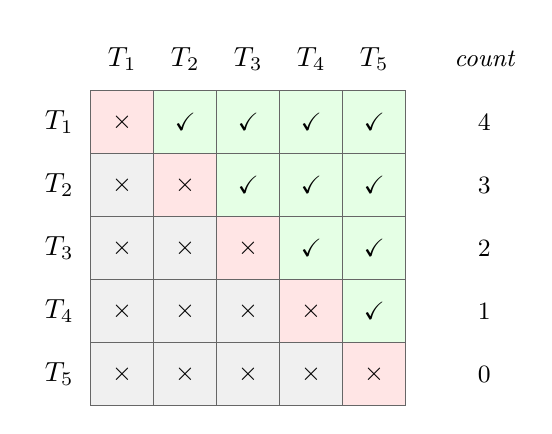
\begin{tikzpicture}[
  every node/.style={font=\small},
  cell/.style={minimum width=8mm, minimum height=8mm, draw=black!60},
  hdr/.style={minimum width=8mm, minimum height=8mm, font=\bfseries},
  diag/.style={cell, fill=red!10},
  lower/.style={cell, fill=gray!12},
  upper/.style={cell, fill=green!10},
]
% column headers
\foreach \j/\name in {1/$T_1$, 2/$T_2$, 3/$T_3$, 4/$T_4$, 5/$T_5$} {
  \node[hdr] at (\j*0.8, 0) {\name};
}
% row headers
\foreach \i/\name in {1/$T_1$, 2/$T_2$, 3/$T_3$, 4/$T_4$, 5/$T_5$} {
  \node[hdr] at (0, -\i*0.8) {\name};
}
% cells: diagonal (red), lower (gray, ✗), upper (green, ✓)
\foreach \i in {1,...,5} {
  \foreach \j in {1,...,5} {
    \ifnum\i=\j
      \node[diag] at (\j*0.8, -\i*0.8) {$\times$};
    \else
      \ifnum\i>\j
        \node[lower] at (\j*0.8, -\i*0.8) {$\times$};
      \else
        \node[upper] at (\j*0.8, -\i*0.8) {$\checkmark$};
      \fi
    \fi
  }
}
% row tally on the right
\foreach \i/\cnt in {1/4, 2/3, 3/2, 4/1, 5/0} {
  \node[font=\small] at (5.4, -\i*0.8) {$\cnt$};
}
\node[font=\small\itshape] at (5.4, -0.0) {count};
\end{tikzpicture}
\end{center}

\textbf{Reading the table.}
\begin{itemize}
  \item \textbf{Diagonal} ($\times$, red): a team cannot play itself.
  \item \textbf{Lower triangle} ($\times$, gray): the pair $(T_i, T_j)$ with $i>j$ records the \emph{same} game as $(T_j, T_i)$, so we strike it out to avoid double-counting.
  \item \textbf{Upper triangle} ($\checkmark$, green): exactly one entry per distinct unordered pair.
\end{itemize}

Counting the checks row by row gives
\[
  4 + 3 + 2 + 1 + 0 \;=\; 10 \text{ games.}
\]

\section*{Approach 2: Row-by-row generalization}

The same table works for any $n$. In row $T_k$, the cell in column $T_j$ is a check exactly when $j > k$, so row $T_k$ contributes $n-k$ unordered pairs.

\begin{tcolorbox}[mybox, title=Key observation]
For row $T_k$, any element up to and including $T_k$ itself cannot be considered: the diagonal cell ($T_k$ playing itself) is excluded, and all cells with $j<k$ are already accounted for in earlier rows. Only the $n-k$ entries with $j>k$ contribute.
\end{tcolorbox}

Summing over all rows:
\[
\begin{aligned}
\text{Total} \;=\; \sum_{k=1}^{n}(n-k)
  &\;=\; \underbrace{(n-1) + (n-2) + \cdots + 1 + 0}_{n \text{ terms}} \\
  &\;=\; \sum_{k=1}^{n} n \;-\; \sum_{k=1}^{n} k \\
  &\;=\; n\cdot n \;-\; \frac{n(n+1)}{2} \\
  &\;=\; \frac{2n^2 - n(n+1)}{2} \;=\; \frac{n(n-1)}{2}.
\end{aligned}
\]

\textbf{Sanity check.} For $n=5$: $\dfrac{5\cdot 4}{2} = 10$. \checkmark

\section*{Approach 3: Count ordered pairs, then divide}

Forget the table. Think of building a pair by filling two labeled slots in sequence:
\[
  \bigl(\ \underline{\ \text{1st}\ }\ ,\ \underline{\ \text{2nd}\ }\ \bigr).
\]

\begin{itemize}
  \item The first slot can be filled in $n$ ways (any element of $S$).
  \item Once the first slot is fixed, the second slot can be filled in $n-1$ ways: any element \emph{except} the one already chosen (since the pair must contain two different elements).
\end{itemize}

Therefore the number of \textbf{ordered} pairs of distinct elements is
\[
  n(n-1).
\]

\begin{tcolorbox}[mybox, title=From ordered to unordered: the division principle]
Each unordered pair $\{s_i, s_j\}$ corresponds to \emph{exactly two} ordered pairs, namely $(s_i, s_j)$ and $(s_j, s_i)$. The count $n(n-1)$ therefore double-counts every unordered pair, and we recover the unordered count by dividing by the size of the symmetry group ($2$):
\[
  \text{unordered pairs} \;=\; \frac{n(n-1)}{2}.
\]
\end{tcolorbox}

This is a special case of a general rule: \emph{when every object is counted the same number of times $m$, divide by $m$.}

\section*{Result}

\begin{tcolorbox}[resultbox, title=Number of unordered pairs from $n$ distinct elements]
\[
  \binom{n}{2} \;=\; \frac{n(n-1)}{2}.
\]

\medskip
For the baseball tournament with $n=5$ teams:
\[
  \binom{5}{2} \;=\; \frac{5\cdot 4}{2} \;=\; 10 \text{ games.}
\]
\end{tcolorbox}

\section*{Cross-check: small values}

\begin{center}
\renewcommand{\arraystretch}{1.2}
\begin{tabular}{@{}cccc@{}}
\toprule
$n$ & Row-sum $\sum_{k=1}^{n}(n-k)$ & Ordered/$2 \,=\, n(n-1)/2$ & $\binom{n}{2}$ \\
\midrule
$2$ & $1+0 = 1$              & $2\cdot 1/2 = 1$    & $1$  \\
$3$ & $2+1+0 = 3$            & $3\cdot 2/2 = 3$    & $3$  \\
$4$ & $3+2+1+0 = 6$          & $4\cdot 3/2 = 6$    & $6$  \\
$5$ & $4+3+2+1+0 = 10$       & $5\cdot 4/2 = 10$   & $10$ \\
$6$ & $5+4+3+2+1+0 = 15$     & $6\cdot 5/2 = 15$   & $15$ \\
\bottomrule
\end{tabular}
\end{center}

All three columns agree, as they must.

\section*{Conclusion}

\begin{tcolorbox}[conclbox, title=Summary]
The number of unordered pairs of distinct elements drawn from an $n$-element set is
\[
  \binom{n}{2} \;=\; \frac{n(n-1)}{2}.
\]
We proved this three ways:
\begin{enumerate}
  \item \textbf{Concrete table} ($n=5$): count check marks in the upper triangle.
  \item \textbf{Row-by-row sum}: row $T_k$ contributes $n-k$ pairs; summing yields $n^2 - \tfrac{n(n+1)}{2} = \tfrac{n(n-1)}{2}$.
  \item \textbf{Division principle}: $n(n-1)$ ordered pairs, each unordered pair counted twice, so divide by $2$.
\end{enumerate}
The three viewpoints — \emph{enumerate carefully}, \emph{sum a pattern}, \emph{overcount and divide} — are the standard combinatorial moves and recur throughout the subject.
\end{tcolorbox}

\vspace{6pt}
\noindent\textit{Remark (where this quantity shows up).} The number $\binom{n}{2}$ counts:
\begin{itemize}
  \item the \emph{edges of the complete graph} $K_n$ on $n$ vertices;
  \item the \emph{handshakes} exchanged when $n$ people each shake hands with every other person once;
  \item the \emph{number of $2$-element subsets} of an $n$-set;
  \item the \emph{$n$-th triangular number} $T_{n-1} = 1 + 2 + \cdots + (n-1)$.
\end{itemize}

\noindent\textit{Remark (generalization).} The third approach extends immediately: the number of unordered $r$-subsets of an $n$-set is
\[
  \binom{n}{r} \;=\; \frac{n(n-1)(n-2)\cdots(n-r+1)}{r!},
\]
obtained by counting ordered $r$-tuples of distinct elements ($n(n-1)\cdots(n-r+1)$ of them) and dividing by the number of orderings of each $r$-subset ($r!$). For $r=2$ this recovers $\tfrac{n(n-1)}{2}$.

\end{document}
